\documentclass[11pt]{article}
\usepackage{amsmath}
\usepackage{amsfonts}
\usepackage{tikz}
\usepackage{circuitikz}
\usepackage{geometry}
\geometry{margin=1in}

\title{Rotational Gear Transfer Function Problem}
\author{ComArchi}
\date{}

\begin{document}

\maketitle

\section{Problem Statement}

Consider a rotational system with two gears connected in series. The system consists of:
\begin{itemize}
    \item Input voltage $V_i$ driving a DC motor
    \item Motor with inertia $J_1$ and damper $D_1$
    \item First gear with $N_1 = 10$ teeth
    \item Second gear with $N_2 = 20$ teeth  
    \item Load with inertia $J_2$ and damper $D_2$
\end{itemize}

Find the overall transfer function relating the output angular position $\theta_2(s)$ to the input voltage $V_i(s)$.

\section{Solution:}

\begin{center}
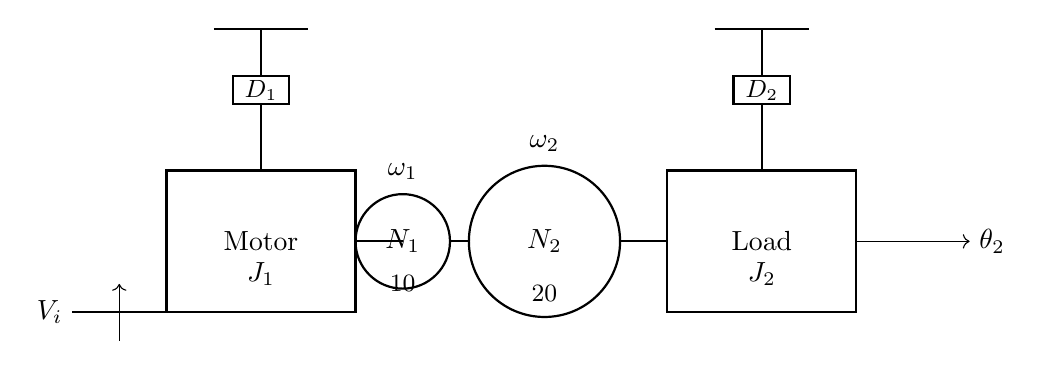
\begin{tikzpicture}[scale=1.2]
    % Input voltage source
    \draw[thick] (0,0) -- (1,0);
    \node[left] at (0,0) {$V_i$};
    \draw[->] (0.5,-0.3) -- (0.5,0.3);
    
    % Motor with inertia J1
    \draw[thick] (1,0) rectangle (3,1.5);
    \node at (2,0.75) {Motor};
    \node at (2,0.4) {$J_1$};
    
    % Damper D1
    \draw[thick] (2,1.5) -- (2,2.2);
    \draw[thick] (1.7,2.2) rectangle (2.3,2.5);
    \node at (2,2.35) {\small $D_1$};
    \draw[thick] (2,2.5) -- (2,3);
    \draw[thick] (1.5,3) -- (2.5,3);
    
    % First gear N1=10
    \draw[thick] (3.5,0.75) circle (0.5);
    \node at (3.5,0.75) {$N_1$};
    \node at (3.5,0.3) {\small 10};
    \draw[thick] (3,0.75) -- (3.5,0.75);
    
    % Second gear N2=20
    \draw[thick] (5,0.75) circle (0.8);
    \node at (5,0.75) {$N_2$};
    \node at (5,0.2) {\small 20};
    \draw[thick] (4,0.75) -- (4.2,0.75);
    
    % Load with inertia J2
    \draw[thick] (6.3,0) rectangle (8.3,1.5);
    \node at (7.3,0.75) {Load};
    \node at (7.3,0.4) {$J_2$};
    \draw[thick] (5.8,0.75) -- (6.3,0.75);
    
    % Damper D2
    \draw[thick] (7.3,1.5) -- (7.3,2.2);
    \draw[thick] (7,2.2) rectangle (7.6,2.5);
    \node at (7.3,2.35) {\small $D_2$};
    \draw[thick] (7.3,2.5) -- (7.3,3);
    \draw[thick] (6.8,3) -- (7.8,3);
    
    % Output angle
    \draw[->] (8.3,0.75) -- (9.5,0.75);
    \node[right] at (9.5,0.75) {$\theta_2$};
    
    % Angular velocities labels
    \node[above] at (3.5,1.3) {$\omega_1$};
    \node[above] at (5,1.6) {$\omega_2$};
    
    % Gear connection
    \draw[thick] (4,0.75) -- (4.2,0.75);
    
\end{tikzpicture}
\end{center}

\vspace{0.5cm}

\textbf{Overall gear ratio:}
\begin{equation}
n = \frac{N_2}{N_1} = \frac{20}{10} = 2
\end{equation}

\textbf{Gear relationships:}
\begin{align}
\omega_2 &= \frac{\omega_1}{n} = \frac{\omega_1}{2}\\
\tau_1 &= n \cdot \tau_2 = 2\tau_2
\end{align}

\textbf{Motor equation:}
\begin{equation}
V_i = K_m \omega_1 + R_m I_m
\end{equation}

\textbf{Torque equations:}
For the motor side (J1):
\begin{equation}
\tau_m - \tau_1 - D_1\omega_1 = J_1 \frac{d\omega_1}{dt}
\end{equation}

For the load side (J2):
\begin{equation}
\tau_2 - D_2\omega_2 = J_2 \frac{d\omega_2}{dt}
\end{equation}

\textbf{Taking Laplace transforms and substituting gear relationships:}

From the motor equation:
\begin{equation}
\tau_m = K_t I_m = \frac{K_t}{R_m}(V_i - K_m \omega_1)
\end{equation}

Substituting into the motor torque equation:
\begin{equation}
\frac{K_t}{R_m}(V_i - K_m \omega_1) - 2\tau_2 - D_1\omega_1 = J_1 s\omega_1
\end{equation}

From the load equation with $\omega_2 = \frac{\omega_1}{2}$:
\begin{equation}
\tau_2 - D_2\frac{\omega_1}{2} = J_2 s\frac{\omega_1}{2}
\end{equation}

Solving for $\tau_2$:
\begin{equation}
\tau_2 = \frac{\omega_1}{2}(D_2 + J_2 s)
\end{equation}

Substituting back into the motor equation:
\begin{equation}
\frac{K_t}{R_m}(V_i - K_m \omega_1) - 2 \cdot \frac{\omega_1}{2}(D_2 + J_2 s) - D_1\omega_1 = J_1 s\omega_1
\end{equation}

Simplifying:
\begin{equation}
\frac{K_t}{R_m}V_i - \frac{K_t K_m}{R_m}\omega_1 - \omega_1(D_2 + J_2 s) - D_1\omega_1 = J_1 s\omega_1
\end{equation}

Collecting terms:
\begin{equation}
\frac{K_t}{R_m}V_i = \omega_1\left[\frac{K_t K_m}{R_m} + D_1 + D_2 + J_2 s + J_1 s\right]
\end{equation}

Therefore:
\begin{equation}
\frac{\omega_1(s)}{V_i(s)} = \frac{\frac{K_t}{R_m}}{\frac{K_t K_m}{R_m} + D_1 + D_2 + s(J_1 + J_2)}
\end{equation}

Since $\theta_2(s) = \frac{\omega_2(s)}{s} = \frac{\omega_1(s)}{2s}$:

\boxed{
\frac{\theta_2(s)}{V_i(s)} = \frac{K_t}{2R_m s[K_t K_m + R_m(D_1 + D_2) + R_m s(J_1 + J_2)]}
}

\end{document}